\documentclass[a4paper, 12pt]{article}
\usepackage[slovene]{babel}
\usepackage[utf8]{inputenc}
\usepackage[T1]{fontenc}
\usepackage{hyperref}
\usepackage{graphicx}
\usepackage[backend=biber]{biblatex}
\usepackage{float}

\addbibresource{viri.bib}

\hypersetup{
	colorlinks,
	citecolor=black,
	filecolor=black,
	linkcolor=black,
	urlcolor=black
}

\begin{document}
	\begin{titlepage}
		\newcommand{\HRule}{\rule{\linewidth}{0.5mm}}
		\center

		\textsc{\LARGE Gimnazija Vič}\\[0.5cm]
		\textsc{\Large Tržaška c. 72, 1000 Ljubljana}\\[0.5cm]
		\textsc{\Large Maturitetna seminarska naloga pri predmetu informatika}\\[1cm]

		\HRule \\[0.4cm]
		{ \huge \bfseries Programiranje za mobilne platforme iOS}\\[0.4cm]
		\HRule \\[1.5cm]

		\begin{minipage}{0.4\textwidth}
			\begin{flushleft} \large
				\emph{Avtor:}\\
				Vid Drobnič
			\end{flushleft}
		\end{minipage}
		~
		\begin{minipage}{0.4\textwidth}
			\begin{flushright} \large
				\emph{Mentor:} \\
				prof. Klemen Bajec
			\end{flushright}
		\end{minipage}\\[4cm]

		{\large februar 2017}\\[3cm]
		\vfill
	\end{titlepage}

	\begin{abstract}
		\noindent Projektna naloga se ukvarja z ravojem aplikacije GimVic za mobilne naprave z operacijskim sistemom iOS. Namen aplikacije je dijakom in profesorjem Gimnazije Vi"c olaj"sati pregledovanje urnika in suplenc. Projektna naloga ima tri dele. Prvi del seminarske naloge se ukvarja z operacijskim sistemom iOS in razvojem aplikacij zanj. Drugi del se ukvarja z samo izdelavo GimVic aplikacije. Ker je aplikacija razmeroma obse"zna, ni primerno, da bi bila predstavljena v celoti, zato so podrobneje razlo"zeni samo nekateri pomembnej"si deli. Tretji del opisuje objavo aplikacije na spletni trgovini AppStore in odziv uporabnikov.\\
		
		\noindent \textbf{Klju"cne besede:} Swift, iOS, AppStore, aplikacija
	\end{abstract}


	\pagebreak

	\tableofcontents
	\pagebreak

	\section{Uvod}
	\paragraph{} Čez celo šolsko leto imamo dijaki veliko nadome"sčanj, ki so dostopna na spletni učilnici. Zaradi nepreglednosti spletne učilnice je pregledovanje nadomeščanj zelo dolgotrajno opravilo. Zato sem se odločil napisati aplikacijo za mobilne naprave z operacijskim sistemom iOS.

\paragraph{} Pred začetkom pisanja aplikacije sem si zadal določene cilje. Poleg prikazovanja urnika z nadomeščanji, sem si kot cilj zastavil tudi prikazovanje jedilnika. Vse zastavljene cilje sem tudi dosegel. Na koncu sem preveril še priljubljenost aplikacije s pomočjo statističnih podatkov, ki sem jih pridobil na Apple-ovi spletni strani za razvijalce.

	\section{Operacijski sistem iOS}
	\paragraph{}iOS\cite{ios-wiki} je Applov operacijski sistem a mobilne naprave. V osnovi je bil zasnovan za iPhone, danes pa ga uporabljajo tudi iPad, iPod Touch in Apple TV. Prva verzija je bila izdana leta 2007. Zasnovan je na Unix-ovem\cite{unix-wiki} jedru.

\subsection{Programiranje za iOS platformo}
\paragraph{}Apple je za iOS razvil razvijalsko orodje Xcode\cite{xcode-wiki}, ki je na voljo za ra"cunalnike z operacijskim sistemom macOS. Naredili so tudi primerno dokumentacijo\cite{ios-docs} za programiranje za iOS in spletno trgovino imenovane App Store\cite{app_store-wiki}, kamor razvijalci objavimo svoje aplikacije.

\subsubsection{Jeziki}
\paragraph{}"Cez leta se je zamenjalo veliko jezikov za pisanje aplikacij za iOS platformo. Prvotno so se aplikacije pisale v C++\cite{cpp-wiki}. Kasneje ga je zamenjal programski jezik Objective-C\cite{objective-c-wiki}, ki je bil uporabljen samo na Applovih platformah. Leta 2014 je Apple predstavil svoj odprtokodni programski jezik imenovan Swift\cite{swift-wiki}, ki naj bi zamenjal sedaj nekoliko zastarel Objective-C\cite{objective-c-wiki}.

\subsubsection{Zgradba iOS Aplikacije}
\paragraph{}Aplikacije za iOS se shranjujejo v Xcode projektih. To je skupina map in datotek z dolo"ceno strukturo. Prevladujejo Swift oziromva Objective-C (odvisno od tega kater jezik si izberemo za razvoj), .storyboard, .xib in .plist datoteke. V .storyboard in .xib datotekah se nahaja zgradba uporabni"skega vmesnika, v .plist datotekah se nahaja konfiguracija aplikacije (ime aplikacije, ime razvijalca, ...), v Swift oziroma Objective-C datotekah pa se nahaja koda, ki se kasneje izvaja na napravi.	

\paragraph{}Aplikacije je sestvaljena na modelu MVC\cite{mvc-wiki} (Model-View-Controller). Model nam predpi"se tri glavne komponente aplikacije. Komponenta Model skrbi za pridobivanje, shranjevanje in obdelavo podatkov, komponenta View skrbi za prikazovanje grafi"cnega vmesnika, komponenta Controller pa povezuje Model in View med seboj. Ko uporabnik pritisne na dolo"ceno del uporabni"skega vmesnika, gre Controller po podatke v Model objekt in nato pove View objektu katere podatke naj prika"ze. 


	\section{Razvoj aplikacije}
	\paragraph{}Da bi bila aplikacija "cim bolj prijazna uporabniku je "sla "cez veliko razli"cic in popravkov. V nadaljevanju je opisano kako deluje trenutno najnovej"sa razli"cica 3.0. Izvorna koda je dostopna na spletnem portalu GitHub na naslovu \url{https://github.com/GimVic-app/gimvic-ios}.

\subsection{Struktura}
\paragraph{}
Aplikacija je sestavljena iz dveh delov. Prvi del se ukvarja s pridobivanjem podatkov iz stre"znika, drugi del pa se ukvarja s predstavitvijo podatkov uporabniku. Del aplikacije, ki se ukvarja s pridobivanjem in shranjevanjem podatkov je narejen kot knji"znica (Framework), ki jo aplikacija uporablja. S tem lahko kasneje dodam "se druge na"cine prikazovanja urnika uporoabniku (na primer gradnik (\textit{ang.} widget)), brez da bi ponovno pisal pridobivanje podatkov.

\subsection{Podatki} 
\paragraph{}Podatki, ki jih aplikacija potrebuje, so servirani iz razli"cnih stre"znikov v razli"cnih oblikah zapisa. Urnik je na voljo v JavaScript Array\cite{js-array} obliki, nadome"s"canja pa v JSON\cite{json-wiki}. Jedilnik za "solsko malico in kosilo se nalo"zi na stre"znik v csv\cite{csv-wiki} obliki. Odlo"cil sem se, da bo za podatke skrbel poseben stre"znik, ki bo vse od zgoraj na"stetega zdru"zil v enovito JSON obliko, ker bo tako prikazovanje na telefonu hitrej"se in bolj u"cinkovito. Stre"znik si podatke shranjuje v MySQL\cite{mysql-wiki} podatkovno bazo\cite{rin} in jih nato servira v JSON obliki.

\paragraph{}Pri dostopu do podatkov stre"zniku z URL parametri\cite{query-string-wiki} poda"s ali "zeli"s podatke za profesorja, ali pa za dijaka. Pri profesorju stre"zniku kot parameter poda"s ime profesorja, pri dijaku pa razred in izbirne ozroma maturitetne predmete. Stre"znik nato vrne seznam, kjer vsak element v tem seznamu predstavlaj podatke za dolo"cen dan v tednu. Vsak dan je predstavljen z seznamom v katerem vsak element predstavlja uro.

\begin{figure}[!h]
	\centering
	Primer URL-ja:
	\texttt{http://gimvicapp.404.si/data?addSubstitutions=true\&classes[]=4B\\\&snackType=navadna\&lunchType=navadno}
\end{figure}

\subsubsection{Upravitelj podatkov}
\paragraph{}
Glaven razred v knji"znici za delo s podatki je upravitelj podatkov, ki skrbi za pridobivanje podatkov iz stre"znika, njihovo obdelovanje in shranjevanje. Za"zene se vsaki"c ko se aplikacija odpre in najprej preveri starost trenutno shranjenih podatkov. "Ce so podatki prestari gre na stre"znik po nove podatke, ki jih pretvori v primerne podatkovne strukture in shrani na pomnilnik telefona. Nato o novih podatkih obvesti glavno aktivnost, ki osve"zi grafi"cni vmesnik z novimi podatki.

\paragraph{}
"Ce upravitelj podatkov ugotovi, da naprava nima internetne povezave uporabi podatke, ki so "ze shranjeni na napravi. Uporabnik lahko podatke osve"zi ro"cno. V tem primeru glavna aktivnost zahteva od upravitelja podatkov, da gre po nove podatke.

\paragraph{}
Upravitelj podatkov je \texttt{singleton}, kar pomeni, da inicializiran samo en objekt, ki ga uporabljajo vsi drugi objekti. S tem se izognemo podvojevanju podatkov in neso"casnega osve"zevanja, zaradi "cesar aplikacija porabi manj spomina in prenese manj podatkov.

\paragraph{}
Vsak objekt, ki "zeli od upravitelja podatkov prejemati sporo"cila o spremembah podatkov, se mora dodati kot delegat (\textit{ang.} delegate). Upravitelj podatkov ima za shranjevanje delegatov mapo (\textit{ang.} dictionary). Vsak delegat je shranjen v mapi pod svojim imenom, ki predstavlja klju"c. S tem se lahko kasneje objekt pri zbrisevanju odstrani iz upravitelja podatkov. 

\begin{center}
	Initializacija singleton objekta in shranjevanje delegatov:
\end{center}
\begin{minted}[frame=lines]{swift}
public final class TimetableData {
  public static let sharedInstance = TimetableData()
	
  public var delegates = [DelegateID: TimetableDataDelegate]()
  ...
}
\end{minted}

\paragraph{}
Ker morajo biti vsi objekti v mapi istega tipa, izkoristimo protokole. V Swiftu s protokolom definiramo, katere funkcije in spremenljivke mora objekt imeti. Protokol se nato obna"sa kot tip spremenljivke. S tem zagovotimo da imajo vsi shranjeni objekti na voljo funkcijo, ki jo kli"cemo, ko se spremenijo podatki.

\begin{minted}[frame=lines]{swift}
public protocol TimetableDataDelegate {
  func timetableDataDidUpdateWithStatus(_ status: DataGetterStatus)
}
\end{minted}

\paragraph{}
Zelo moramo paziti, da se vsak objekt, ki se doda kot delegat, tudi odstrani. Druga"ce lahko do objekta dostopamo preko ve"ceih kazalcev (pointer), kar pomeni, da se objekt nikoli ne bo odstranil iz pomnilnika. S tem ustvarimo pu"s"canje pomnilnika (\textit{ang.} memory leak).

\subsection{Predstavitev podatkov}
Del aplikacije, ki skrbi za predstavitev podatkov uporabniku, je sestavljen iz ve"cih komponent:
\begin{itemize}
	\setlength\itemsep{0em}
	\item glavna aktivnost (\textit{ang.} root view controller) (slika \ref{fig:main_view})
	\item nastavitve (slika \ref{fig:settings})
	\item o aplikaciji
\end{itemize}

\begin{figure}[!h]
	\begin{minipage}{0.45\linewidth}
		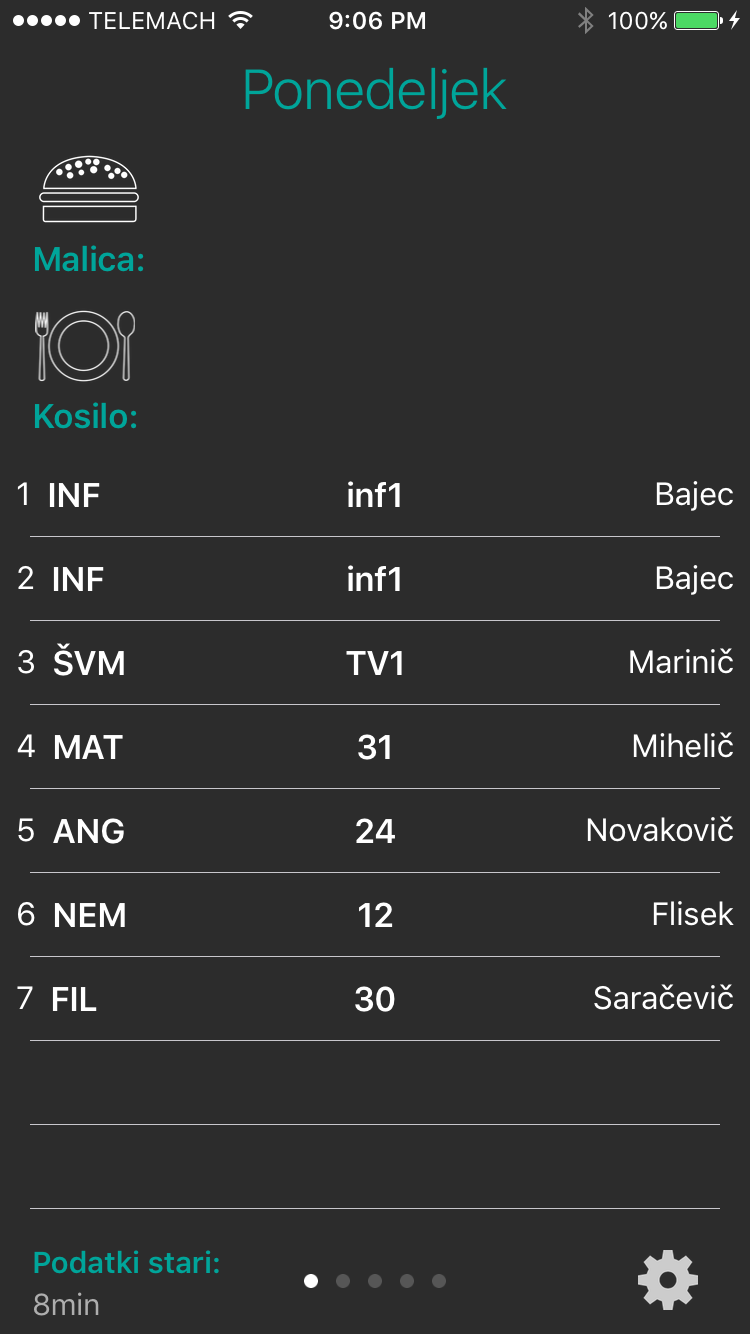
\includegraphics[width=\linewidth]{images/main_view.png}
		\caption{Glavna aktivnost}\label{fig:main_view}
	\end{minipage}\hfill
	\begin{minipage}{0.45\linewidth}
		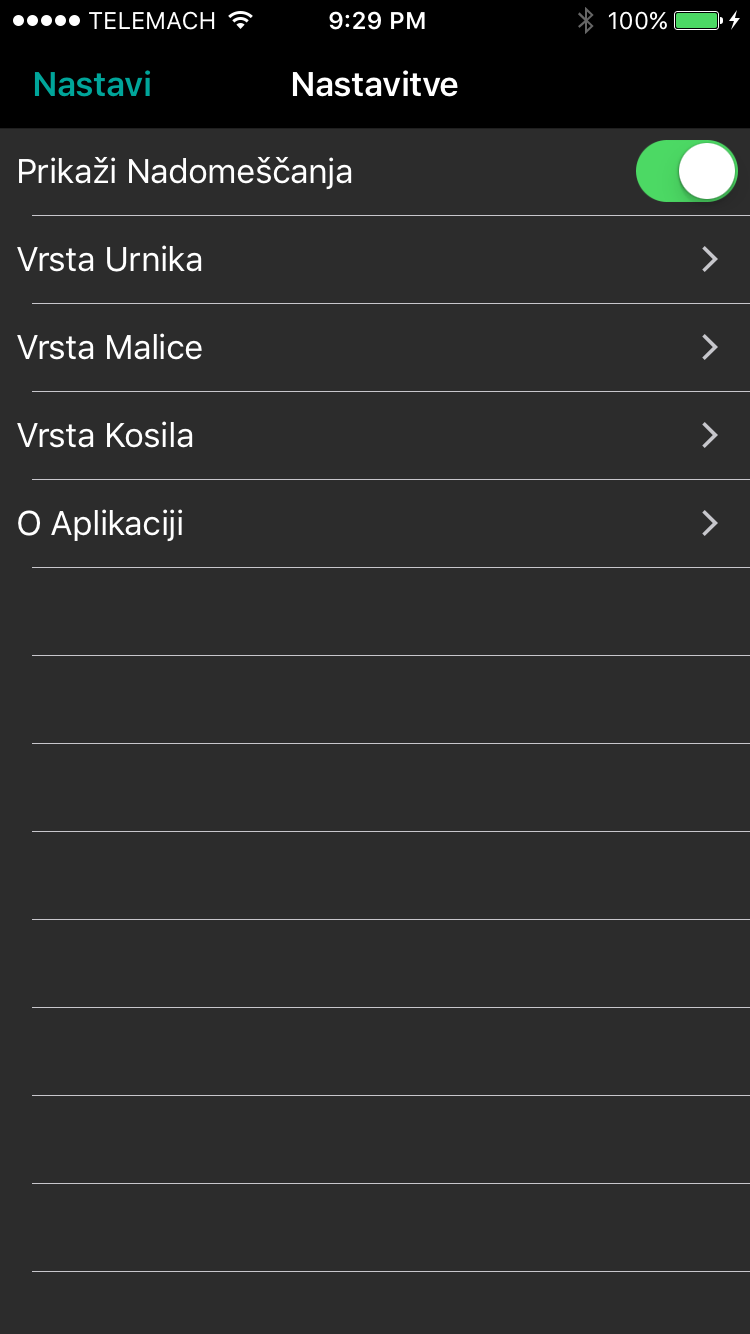
\includegraphics[width=\linewidth]{images/nastavitve.png}
		\caption{Nastavitve}\label{fig:settings}
	\end{minipage}
\end{figure}

\subsubsection{Glavna aktivnost}
\paragraph{}Tu se odvija ve"cino uporabniku pomembnih stvari. Ko uporabnik odpre aplikacijo se mu prika"ze glavni pogled (\textit{ang.} main view) (slika \ref{fig:main_view}) v katerem je za vsak dan prikazan jedilnik in urnik. V glavni aktivnosti se nahaja tudi gumb za nastavitve.

\paragraph{}Ko se aplikacija odpre, najprej preveri, "ce je odprta prvi"c. V tem primeru uporabnika popelje "cez osnovne nastavitve kjer nastavi razred oziroma ime profesorja, ter vrsto malice in kosila. 

\begin{minted}[frame=lines]{swift}
override func viewDidAppear(_ animated: Bool) {
  super.viewDidAppear(animated)

  if UserDefaults().object(forKey:
                           UserSettings.
                           lastRefreshedTimetableData.
                           rawValue) as? Date == nil {
    let setupStoryboard = UIStoryboard(name: "Setup", bundle: nil)
    let viewController = setupStoryboard.instantiateInitialViewController()!
    present(viewController, animated: true, completion: nil)
  }
}
\end{minted}

\paragraph{}
Aplikacija nato prika"ze vse elemente uporabni"ska vmesnika. V osnovi je sestavljen iz \texttt{UIScrollView}-ja, ki skrbi zato, da se lahko premikamo levo in desno. \texttt{UIScrollView} ima ve"c otrok, kjer vsak otrok predstavlja pogled(\texttt{UIView}) za en dan v tednu. Otrok ima eno tekstovno polje (\texttt{UILabel}) v katerem je zapisan dan v tednu in "se dve tekstovni polji v katerih sta zapisana malica in kosilo. Vsak dnevni pogled vsebuje tudi tabelo (\texttt{UITableView}), v kateri je prikazan urnik.

\paragraph{}
V glavni aktivnosti sta prikazana tudi gumb (\texttt{UIButton}) za nastavitve in kako stari so podatki. Starost podatkov nastavimo, ko se aplikacija prika"ze na zaslon. Nato naredimo nov merilnik "casa (\texttt{NSTimer}), ki vsako minuto kli"ce dolo"ceno funkcijo, ki posodobi starost podatkov.

\begin{minted}[frame=lines]{swift}
func setDataAgeLabel() {
  let lastRefreshed = UserDefaults().
                      object(forKey:
                             UserSettings.
                             lastRefreshedTimetableData.
                             rawValue) as? Date
  if lastRefreshed == nil {
    dataAgeLabel.text = "N/A"
  } else {
    let ageText = FuzzyDate.timeSince(lastRefreshed!)
    dataAgeLabel.text = ageText
  }
}
\end{minted}

\subsubsection{Nastavitve}
\paragraph{}V nastavitvah (slika \ref{fig:settings}) lahko uprabnik nastavi ali je dijak, ali profesor in temu primeren filter za urnik. Nastavi lahko tudi vrsto malice in kosila na katerega je naro"cen. Poleg tega ima tudi mo"znost, da izklopi funkcijo za prikaz nadome"s"canj, tako da je uporabniku prikazan samo urnik. V nastavitvah lahko uporabnik tudi pogleda podatke o aplikaciji.

\paragraph{}
Nastavitve se na zaslon prika"zejo kot modalno okno (\textit{ang.} Modal View). Ko uporabnik zapre nastavitve z pritiskom na gump \textit{Nastavi}, nastavitve sporo"cijo upravitelju podatkov, naj gre po nove podatke.

\begin{center}
	Izhod iz nastavitev:
\end{center}
\begin{minted}[frame=lines]{swift}
@IBAction func doneButtonPressed(_ sender: AnyObject) {
  UserDefaults().synchronize()
  TimetableData.sharedInstance.update()
  navigationController?.dismiss(animated: true, completion: nil)
}
\end{minted}


\subsubsection{O aplikaciji}
\paragraph{}V tem meniju se uporabniku prika"zejo osnovne informacije o aplikaciji kot so avtor aplikacije, verzija in pod katero licenco\cite{license-wiki} je aplikacija izdana. Prav tako je v tem meniju zapisan vir nekaterih ikon, ki so uporabljene, saj to predpisuje licenca pod katero so izdane te ikone.


	\section{Objava aplikacije}
	\paragraph{}Ko sem aplikacijo dokon"cal, sem jo "se objavil v spletni trgovini App Store. Gre virtualno trgovino po kateri uporabniki iOS pregledujejo razli"cne aplikacije in jih nalo"zijo na svoje naprave 

\paragraph{}Za objavo aplikacije na App Store potrebujemo razvijalski ra"cun za Applove naprave, s katerim se prijavimo v njihov spletni portal. Tam naredimo novo aplikacijo in jim dodelimo unikatno ime, ki ga vidi samo razvijalec (\textit{npr.} com.gimvic.ios). Aplikaciji dodamo tudi slike in opis, lahko pa nalo"zimo tudi promocijski video.

\paragraph{}Pred objavo moramo na razvijalski portal nalo"ziti tudi samo aplikacijo - to je datoteka, ki se dejansko izvaja na napravi. To naredimo preko razvijalskega orodja XCode, v katerem smo aplikacijo tudi napisali. V XCode moramo biti prijavljeni z razvijalskim ra"cunom, v konfiguraciji pa mora imeti aplikacija isto unikatno ime, kot smo ji ga dodelili v spletnem portalu. Nato lahko z gumbom publish aplikacijo nalo"zimo na portal.

	\section{Odziv uporabnikov}
	 \paragraph{}Applov spletni portal omogo"ca analizo statisti"cnih podatkov o aplikiciji. To vkju"cuje "stevilo namestitev na naprave, "stevilo aktivnih uporabnikov in pa tudi podatke bolj pomembne za ravijalce, kot so "stevilo zru"sitev aplikacije.
 
 \paragraph{}Trenutno ima aplikacija 139 prenosov. Do velike spremembe bo pri"slo na za"cetku "solskega leta, ko bodo novi dijaki nalo"zili aplikacijo.

	\section{Zaklju"cek}
	\paragraph{}Aplikacijo GimVic za iOS uporabnike sem napisal z namenom, da bi profesorjem in djakom Gimnazije Vi"c olaj"sal pregledovanje urnika, nadome"s"canj in jedilnika. Aplikacija iz stre"znika dobiva realne podatke in jih nato prika"ze uporabniku na prijazen in uporaben na"cin. Dostopna je vsem uporabnikom iOS naprav na spletni trgovini App Store.

\paragraph{}Glede na to, da si je aplikacijo preneslo ve"cino profesorjev in dijakov z iOS napravo in jo tudi aktivno uporabljajo, sem dosegel zastavljen cilj. Prav tako sem zelo zadovoljen z pozitivnim odzivom uporabnikov aplikacije. Sama aplikacija ima "se nekaj manj"sih napak, ki jih bom v prihodnosti popravil.


	\newpage
	\section{Literatura}
	\printbibliography[heading=none]
\end{document}
